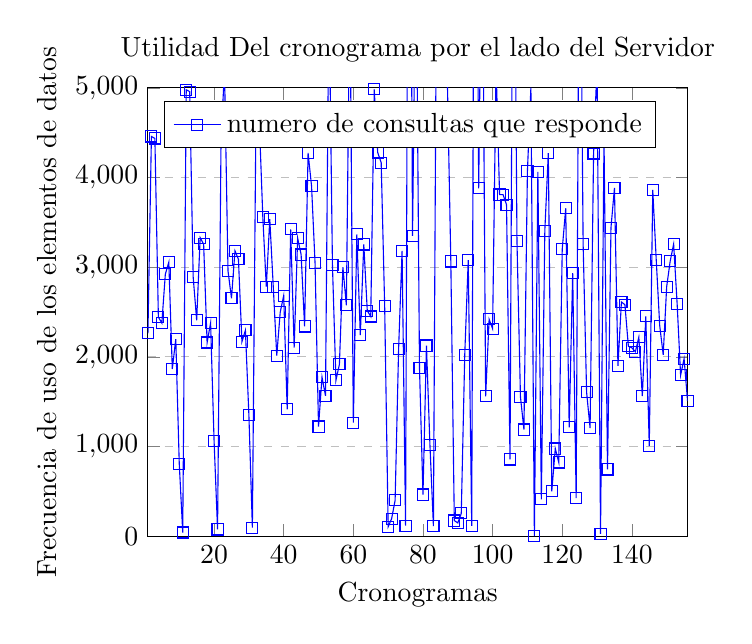
\begin{tikzpicture}
\begin{axis}[
    title={Utilidad Del cronograma por el lado del Servidor},
    xlabel={Cronogramas},
    ylabel={Frecuencia de uso de los elementos de datos},
    xmin=1, xmax=156,
    ymin=0, ymax=5000,
    xtick={},
    ytick={},
    legend pos=north west,
    ymajorgrids=true,
    grid style=dashed,
]

\addplot[
    color=blue,
    mark=square,
    ]
    coordinates {
%UTILIDAD TOTAL
(1,2262)
(2,4458)
(3,4436)
(4,2444)
(5,2377)
(6,2922)
(7,3056)
(8,1865)
(9,2198)
(10,807)
(11,41)
(12,4979)
(13,4958)
(14,2889)
(15,2408)
(16,3329)
(17,3257)
(18,2160)
(19,2378)
(20,1062)
(21,75)
(22,4434)
(23,5199)
(24,2959)
(25,2654)
(26,3183)
(27,3088)
(28,2168)
(29,2296)
(30,1350)
(31,95)
(32,4564)
(33,4617)
(34,3560)
(35,2783)
(36,3537)
(37,2783)
(38,2014)
(39,2498)
(40,2683)
(41,1414)
(42,3423)
(43,2103)
(44,3325)
(45,3141)
(46,2339)
(47,4274)
(48,3904)
(49,3050)
(50,1223)
(51,1774)
(52,1566)
(53,6103)
(54,3021)
(55,1738)
(56,1917)
(57,3000)
(58,2575)
(59,6230)
(60,1266)
(61,3366)
(62,2243)
(63,3254)
(64,2516)
(65,2450)
(66,4983)
(67,4279)
(68,4166)
(69,2563)
(70,105)
(71,196)
(72,400)
(73,2086)
(74,3183)
(75,118)
(76,10806)
(77,3349)
(78,6820)
(79,1874)
(80,464)
(81,2126)
(82,1019)
(83,112)
(84,7118)
(85,5078)
(86,6721)
(87,5096)
(88,3064)
(89,174)
(90,148)
(91,254)
(92,2023)
(93,3080)
(94,116)
(95,11018)
(96,3880)
(97,7296)
(98,1560)
(99,2419)
(100,2314)
(101,5235)
(102,3810)
(103,3809)
(104,3697)
(105,856)
(106,8531)
(107,3289)
(108,1554)
(109,1189)
(110,4071)
(111,5003)
(112,0)
(113,4064)
(114,411)
(115,3406)
(116,4273)
(117,500)
(118,977)
(119,822)
(120,3201)
(121,3657)
(122,1215)
(123,2935)
(124,424)
(125,7917)
(126,3261)
(127,1605)
(128,1205)
(129,4268)
(130,5260)
(131,27)
(132,4432)
(133,744)
(134,3441)
(135,3884)
(136,1900)
(137,2612)
(138,2582)
(139,2118)
(140,2101)
(141,2057)
(142,2219)
(143,1562)
(144,2452)
(145,1005)
(146,3862)
(147,3081)
(148,2347)
(149,2023)
(150,2783)
(151,3066)
(152,3258)
(153,2594)
(154,1795)
(155,1979)
(156,1506)
    };
    \legend{numero de consultas que responde}

\end{axis}
\end{tikzpicture}

